\section{Projektorganisation}

% Wie sind wir vorgegangen... auf alles bezogen. Wer hat an welchen Kapiteln mitgearbeitet.

%Thomas
% ? Während der Projektgruppe haben sich ... Untergruppen/Teams für die jeweiligen Bereiche ... herausgestellt.

Im Rahmen der Projektgruppe 649 nehmen insgesamt 12 Teilnehmer an der Planung und Entwicklung des prozedural generierten 3D Rollenspiels teil. 

Für die Umsetzung des Projektes ist es vorgesehen die verschiedenen Bereiche des Rollenspiels aufzuteilen.

Um ein grundlegendes Verständnis aller Teilnehmenden für alle Bereiche zu schaffen, werden zu Beginn der Projektgruppe in einer Seminarphase alle Bereiche auf Kleingruppen, bestehend aus 3 Teilnehmern, aufgeteilt und potentielle Ansätze für die Umsetzung der Gebiete für ein Videospiel erforscht. Während dieser Seminarphase werden nacheinander die Themen der Gruppen den restlichen Teilnehmenden vorgestellt. Somit wird eine Verständnisgrundlage für alle Beteiligten geschaffen, sodass basierend auf dem allgemeinen Kenntnisstand mit der eigentlichen Entwicklung des Spieles angefangen wird. 

Um anschließend koordiniert das Ziel der Projektgruppe zu erreichen, spielt die Projektorganisation bei einer Gruppe von 12 Teilnehmern eine wichtige Rolle. Im Laufe der Projektgruppe werden Untergruppen gebildet und arbeiten parallel an den verschiedenen Bereichen. Außerdem übernehmen einige Teilnehmer Rollen im Rahmen der Projektleitung. Die primäre Gruppenaufteilung ist in Tabelle \ref{tab:gruppenaufteilung} abgebildet. Initial wird die Projektgruppe in die Untergruppen Creature-Generation und Creature-Animation aufgeteilt.

\begin{itemize}
	\item \textbf{Creature-Generation: } Die Creature-Generation Gruppe wendet verschiedene Methoden der prozeduralen Inhaltsgenerierung an. Damit sollen Skelette für Kreaturen generiert werden und auf Basis dieser Skelette Skinning hinzugefügt werden. Außerdem ist die Creature-Generation Gruppe für die prozedurale Generierung einer Spielwelt verantwortlich.
	\item \textbf{Creature-Animation: } Die Creature-Animation Gruppe wendet Reinforcement Learning an, um Bewegungsmodelle für die von der Creature-Generation Gruppe generierten Kreaturen zu trainieren. 
\end{itemize}

Die weitere Organisation innerhalb der Untergruppen wird in den Abschnitten \ref{subsec:creature-generation-orga} und \ref{sec:creature-animation-orga} genauer beschrieben.

\begin{table}[]
	\centering
	\begin{tabular}{c | c || c | c}
		\multicolumn{2}{c||}{(Creature-)Generation} & \multicolumn{2}{c}{(Creature-)Animation}\\
		\hline
		Creature-Generation & Terrain-Generation & Creature-Animation & neroRL\\
		\hline\hline
		\dotuline{Leonard Fricke} & Kay Heider & Jan Beier & Niklas Haldorn\\
		Jona Lukas Heinrichs& Tom Voellmer & Nils Dunker & \dotuline{Jannik Stadtler}\\
		\dotuline{Mathieu Herkersdorf} & & \dotuline{Carsten Kellner}\\
		Markus Mügge&\\ 
		\underline{Thomas Rysch} &\\    
		
	\end{tabular}
	\caption{Primäre Gruppenaufteilung der Projektgruppe}
	\label{tab:gruppenaufteilung}
\end{table}

\paragraph{Projektleitung}
Aus den initialen Gruppen, der Creature-Generation und der Creature-Animation Gruppe, sind jeweils zwei Projektmanager einberufen. Diese sind in Tabelle \ref{tab:gruppenaufteilung} gepunktet unterstrichen. Außerdem ist Thomas Rysch als Projektleiter ernannt. Der Projektleiter soll darin eine Moderator- und Organisationsrolle einnehmen, die Gruppen und Themen zusammen- und im Überblick behalten und somit potentielle Konflikte frühzeitig erkennen und auflösen. Die Projektmanager übernehmen eine analoge Aufgabe im Rahmen ihrer jeweiligen Gruppen und bilden somit gemeinsam mit dem Projektleiter eine Struktur in der die Übersicht über aktuelle Themen einfach beibehalten werden kann.

\paragraph{Jour-Fixe}
Wöchentlich findet ein Jour-Fixe statt um gemeinsam über die aktuellen Entwicklungen zu sprechen und Herausforderungen gemeinsam anzugehen und zu lösen. Im Anschluss an das Jour-Fixe treffen sich die vier Projektmanager und der Projektleiter, bereiten für den nächsten Termin des Jour-Fixe die zu besprechenden Themen vor und klären gegebenenfalls organisatorische Einzelheiten um somit die restliche Gruppe der Teilnehmer zu entlasten. Während der Jour-Fixe wird von jedem der Teilnehmer abwechselnd eine Dokumentation des Treffens manifestiert um somit Ergebnisse aber auch ToDo's festhalten und einsehen zu können. Für das wöchentliche Treffen wird ein Tagesprotokoll (Fig. \ref{fig:Tagesprotokoll}) genutzt, welches von dem Projektleiter durch Bildschirmübertragung an die Teilnehmer präsentiert und durchgesprochen wird. Das Tagesprotokoll kann jederzeit durch jeden Teilnehmer modifiziert und ergänzt werden, falls zu besprechende Themen durch den jeweiligen Teilnehmer aufgekommen sind.

\begin{figure}[ht]
	\centering
	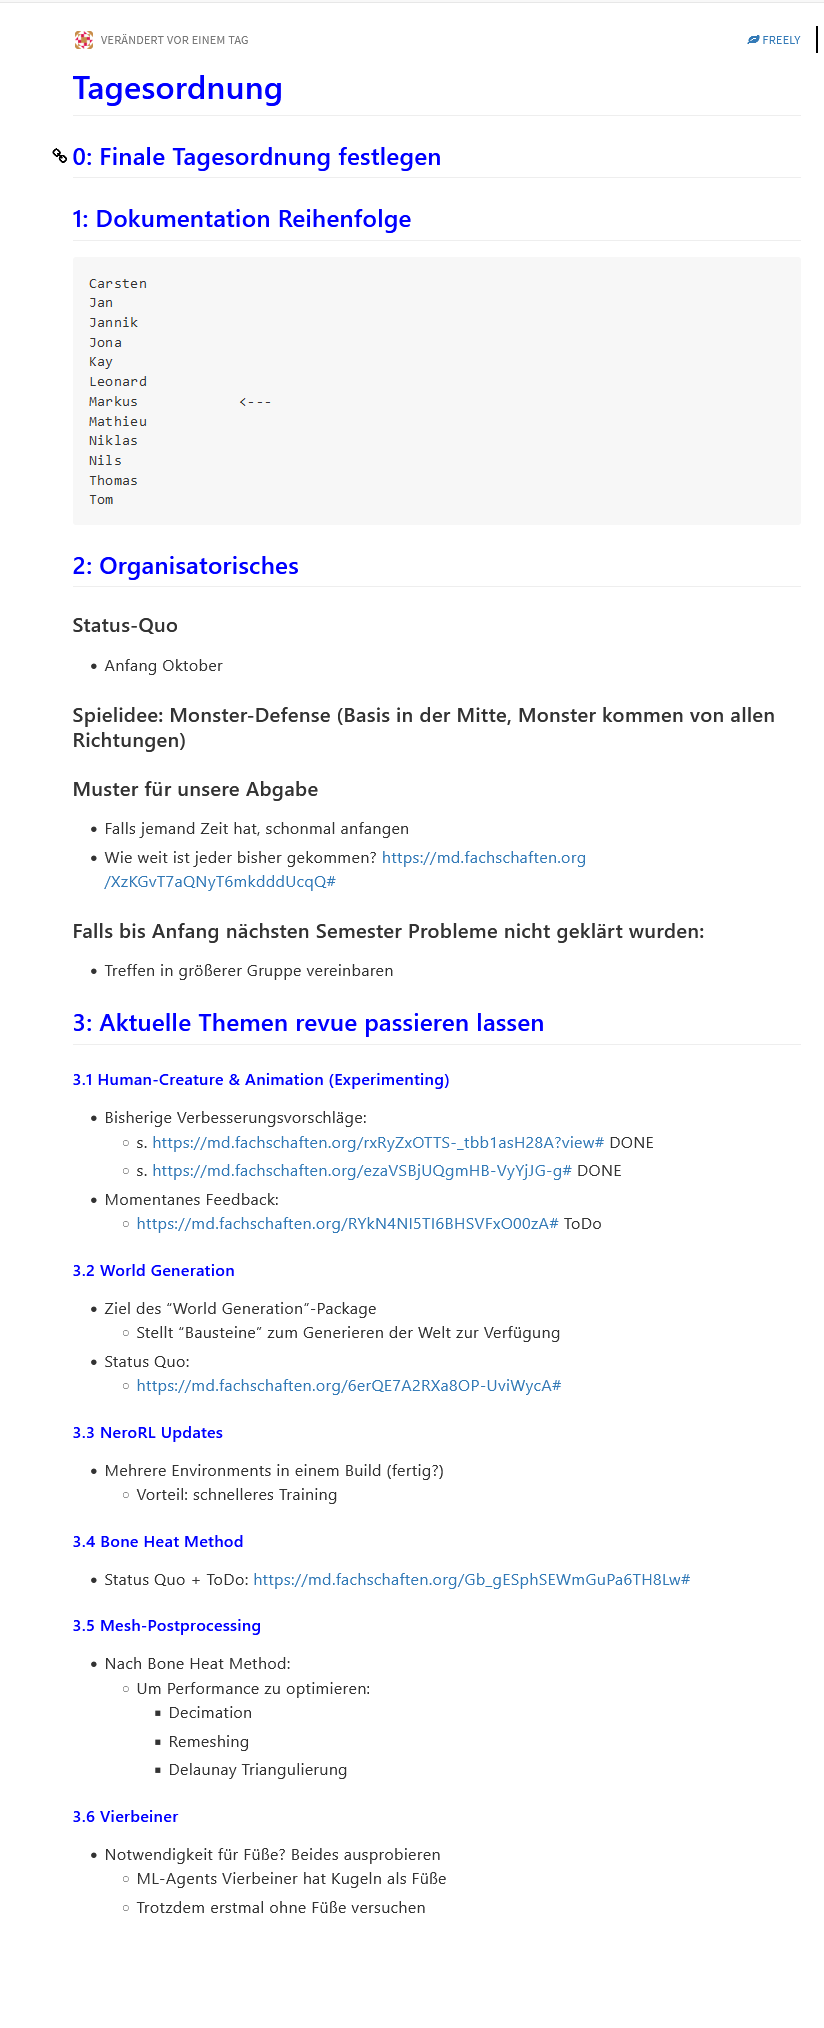
\includegraphics[width=0.5\linewidth]{resources/img/Tagesprotokoll_Beispiel.png}
	\caption{Tagesprotokoll, Stand des 04.10.2022}\label{fig:Tagesprotokoll}
\end{figure}

\paragraph{Organisationswerkzeuge}
Für die weitere Organisation (der Entwicklung und Implementierung) der Projektgruppe werden verschiedene Tools und Hilfsmittel eingesetzt, die im Folgenden beschrieben werden.

\begin{itemize}
	\item \textbf{Discord: } Discord soll als Basis-Kommunikationsmittel genutzt werden. Hier werden für die entsprechenden Phasen und Themenbereiche, sowie Gruppen eigene Text- und Sprach-Kanäle erstellt (Fig. \ref{fig:discord}) Hier werden auch aktuelle (organisatorische-) Themen aufgegriffen und besprochen. Der wöchentliche Jour-Fixe Termin ist ebenfalls in Discord abgehalten.
	\begin{figure}
		\centering
		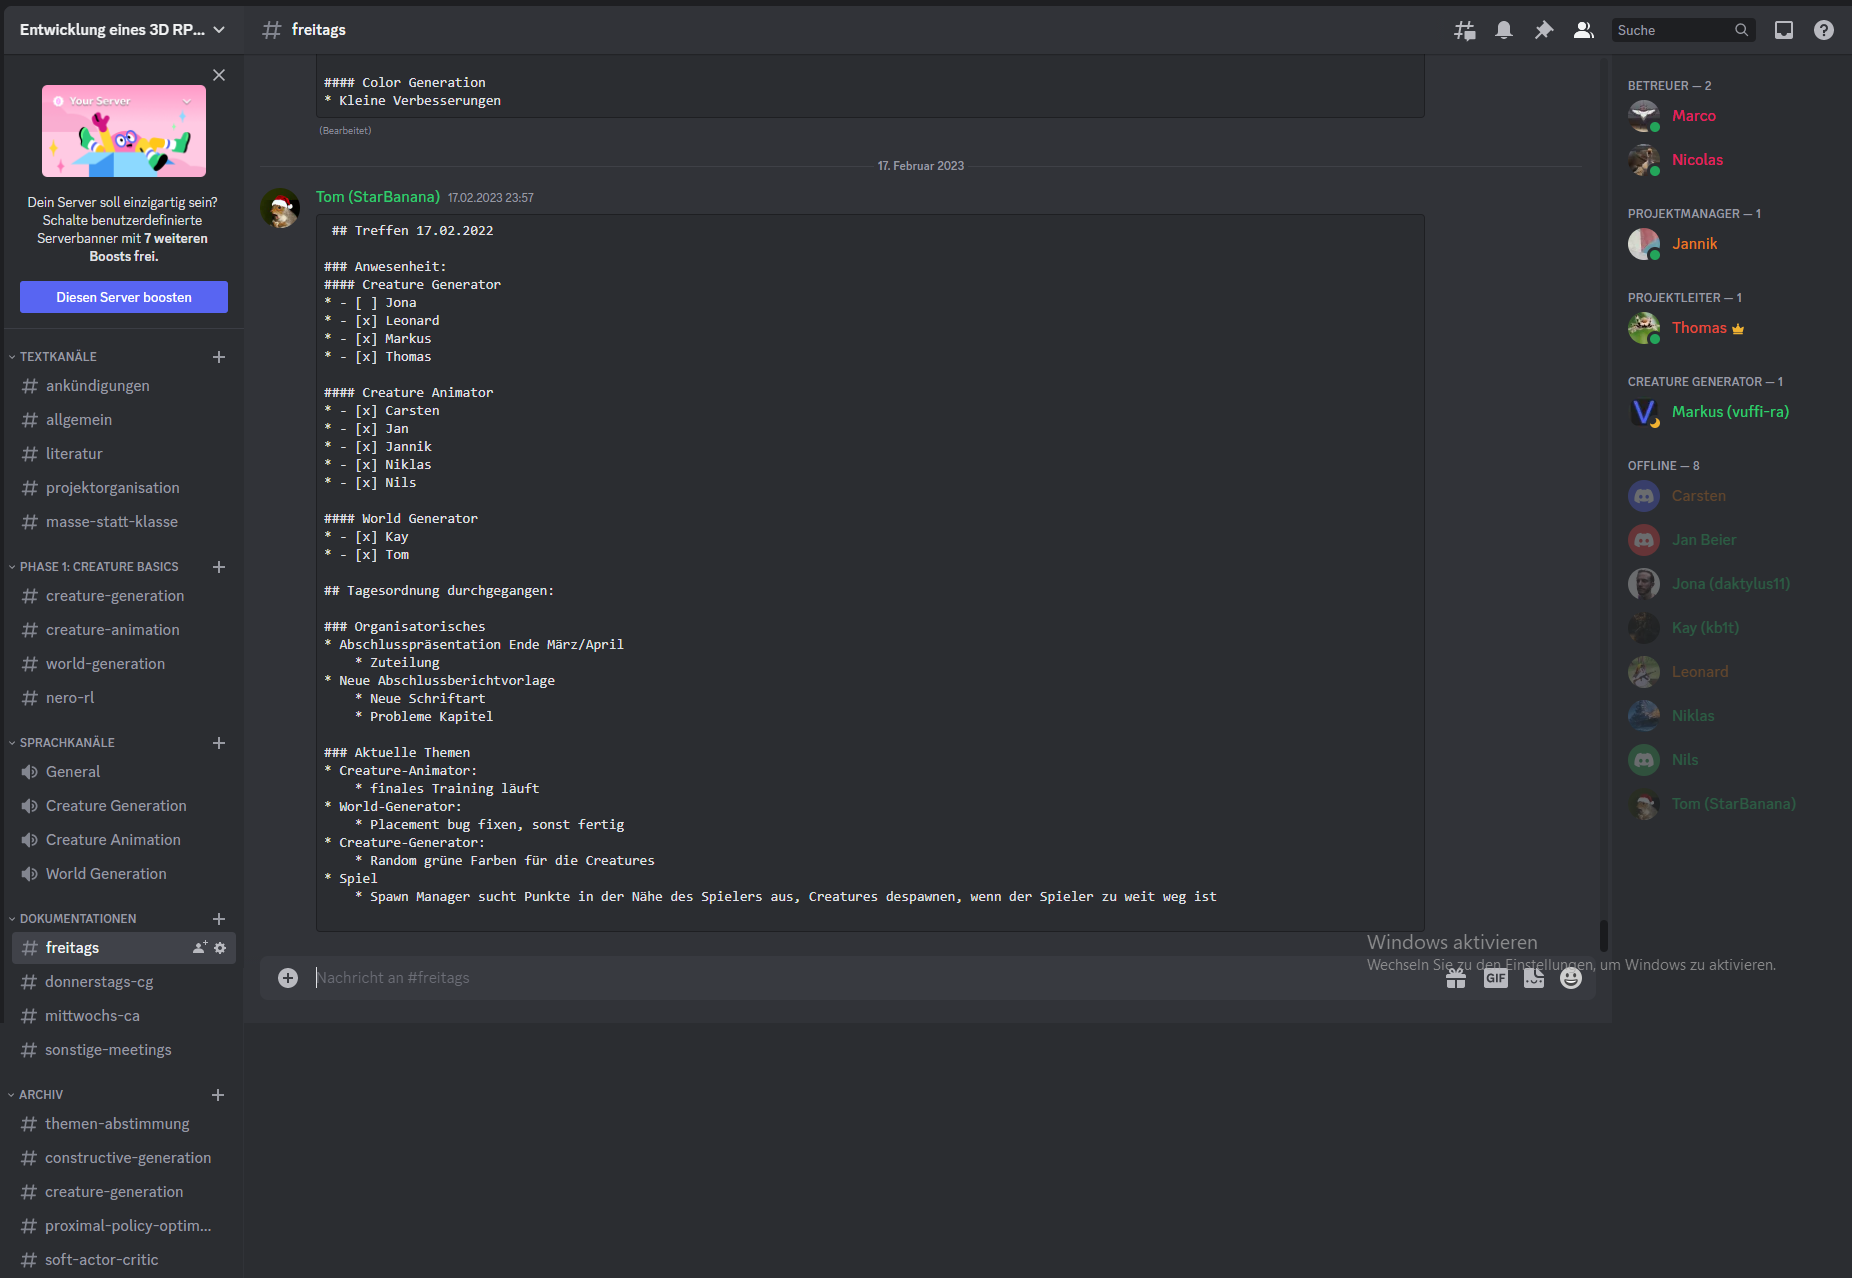
\includegraphics[width=0.7\linewidth]{resources/img/Discord.png}
		\caption{Discord am 27.02.2023}
		\label{fig:discord}
	\end{figure}
	\item \textbf{GitHub: } GitHub wird als Entwicklungs-, Repository- und Speicherplattform genutzt. Die Dokumentationen des wöchentlichen Jour-Fixe sind im GitHub-Wiki abgelegt und zusätzlich in einem Discord Textkanal gespeichert. Somit wird implizit auch durch die Verfügbarkeit auf zwei Plattformen ein Backup der Dokumentationen realisiert, falls im worst-case eine der beiden Plattformen ausfallen sollte. Für die Projektgruppe wird eine GitHub-Organisation gegründet (\href{https://github.com/PG649-3D-RPG}{Link zur Organisation}). Pro Gruppe bzw. Themenbereich soll zunächst ein Repository erstellt werden. Nach Fertigstellung einzelner Versionen werden diese als Pakete exportiert und in einem Main-Repository (\href{https://github.com/PG649-3D-RPG/Horror-Survival-RPG}{Link}) zum fertigen Spiel zusammengestellt.
	\item \textbf{Google-Kalender: } Um insbesondere in der vorlesungsfreien Zeit eine reibungslose Organisation und Ressourcenallozierung gewährleisten zu können, wird Google-Kalender genutzt, in dem sich alle Teilnehmenden in einem Kalender sammeln und ihre jeweiligen Universitäts- und Urlaubsbezogenen Termine eintragen.
	\item \textbf{Status-Quo-Übersicht: } In der Anfangszeit der Projektgruppe hat sich herausgestellt, dass nur schwierig der Überblick über den Gesamtfortschritt der Projektgruppe zu halten ist. Um den Fortschritt insbesondere auch außerhalb der Projektorganisation zu festzuhalten, wird ein Status-Quo Dokument entwickelt. Dieses stellt bereits fertiggestellte, momentan laufende und potentiell in Zukunft zu behandelnde Projekte und Themengebiete übersichtlich dar. Dafür wird mit Hilfe des Tools Graphviz (Fig. \ref{fig:status-quo}) ein simpler Graphen erzeugt der zudem am Anfang jedes Monats durch die Management-Runde aktuell gehalten werden soll. Abbildung \ref{fig:status-quo} zeigt den Status-Quo zum Zeitpunkt der Erstellung des Abschlussberichtes.
	\begin{figure}
		\centering
		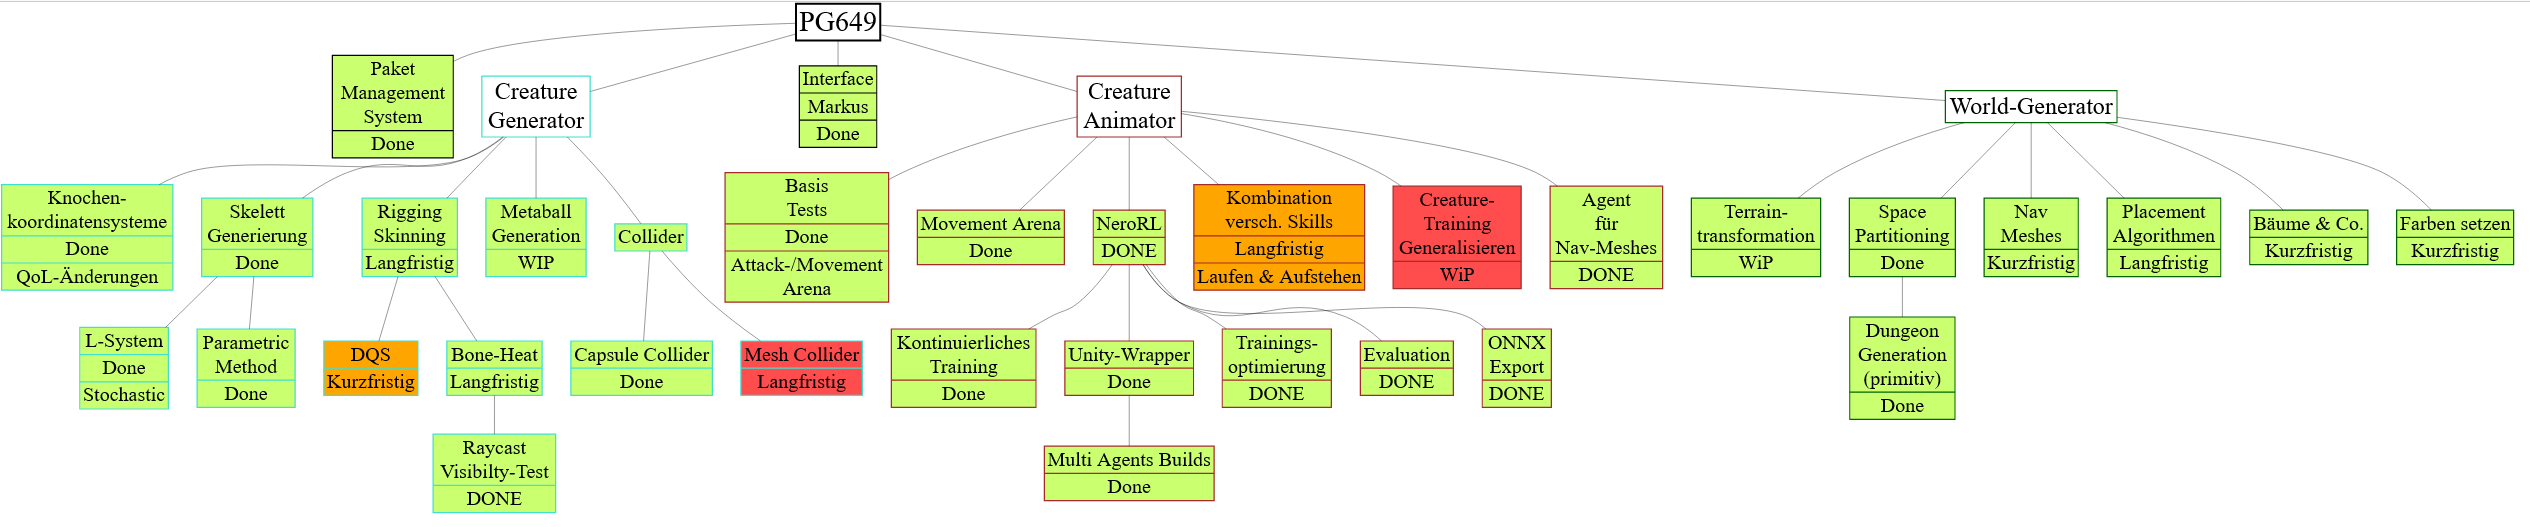
\includegraphics[width=0.7\linewidth]{resources/img/Graphviz_fin.png}
		\caption{Stand des (fertigen) Status-Quo am 26.02.2023}
		\label{fig:status-quo}
	\end{figure}
	\item \textbf{Projekt-Timeline: } Zu Beginn der Projektgruppe wird eine Projekt-Timeline erstellt, welche für das jeweilige Semester die kurz- und langfristigen Aufgaben der entsprechenden Gruppen in tabellarischer Form festhalten soll. Da dieses Hilfsmittel jedoch in dem ersten Semester keine Verwendung fand, wird es zu Anfang der zweiten Hälfte der Projektgruppe als obsolet eingestuft und verworfen. Die kurz- und langfristigen Aufgaben werden stattdessen über das Status-Quo Dokument und die wöchentlichen Jour-Fixe Dokumentationen festgehalten.
\end{itemize}



\subsection{Creature Generator}
\label{subsec:creature-generation-orga}

In der ersten Phase hat sich die Creature-Generation Gruppe mit der Evaluation und Findung eines geeigneten Generator-Algorithmus beschäftigt. Zunächst werden dafür in zwei temporären Untergruppen zwei verschiedene Ansätze erforscht:

\paragraph{Skelett $\rightarrow$ Skin} Bei dem ersten Ansatz wird mit einem L-System Parser experimentiert, zuerst Koordinaten zu erzeugen und das Skelett der Kreatur dann dort reinzulegen (s. Kapitel \ref{L_System}). Der Skin der Kreatur sollte dabei über Metaballs (Kapitel \ref{Metaball_Gen}) und Marching Cubes (Kapitel \ref{Marching_Cubes}) zusammengestellt werden.

\paragraph{Skin $\rightarrow$ Skelett} Bei dieser Alternative soll mit Hilfe von Metaballs und Marching Cubes zuerst ein Skin erzeugt werden, in welches dann ein Skelett durch Automatic Rigging reingelegt werden und durch Dual Quaternion Skinning animierbar gemacht werden soll. Während der Ausarbeitung trifft sich die Creature-Generator Gruppe wöchentlich am Mittwoch und hält analog zum wöchentlichen Jour-Fixe aller Teilnehmer einen Regeltermin zum Besprechen von abgeschlossenen aber auch ausstehenden Aufgaben ab. Eine Dokumentation davon wird ebenfalls analog zum Jour-Fixe sowohl auf Discord als auch im GitHub-Wiki des Creature-Generation Repositories (Link TODO) abgelegt. Am Schluss der Evaluation beider Ansätze wurde sich für die erste Alternative entschieden: es soll das L-System zum Erzeugen der initialen Koordinaten genutzt werden, um daraus dann das Skelett zu erstellen und anschließend mit Hilfe der Metaballs den Skin über das Skelett zu legen. Der Dual Quaternion Ansatz (Kapitel TODO) wird fortwirkend von Leonard Fricke weiterverfolgt, hat jedoch zu diesem Zeitpunkt noch keine große Priorität, da das erste Ziel eine funktionierende Skelett Generierung zu erhalten ist, um sich danach dem Skin-Mesh widmen zu können. Während der weiteren Ausarbeitung hat sich jedoch ein Alternativansatz zum L-System von Jona Heinrichs gezeigt (Kapitel TODO), um effizientere Skelette erzeugen zu können. Damit wird die Entwicklung des L-Systems an dieser Stelle eingestellt. Somit wird entschieden, dass beide Autoren des L-Systems, Tom Voellmer und Kay Heider, von der Creature-Generation Gruppe in eine weitere Gruppe der Terrain-Generator abgezweigt werden, da sich beide Teilnehmer während der Seminarphase mit der Terrain-Generation beschäftigt haben und somit das nächste Thema angehen. Inzwischen wurden an die Creature-Animator Gruppe bereits erste Skelette als Blueprints bereitgestellt, sodass diese bereits ihr Training auf den bis zu diesem Zeitpunkt erzeugten Kreaturen prüfen konnten. Dabei hat sich Markus Mügge als Vermittler zwischen den Creature-Generatorn und Creature-Animatorn bereiterklärt und ist somit für die Kommunikation und den Wissensaustausch beider Teams außerhalb der Jour-Fixe zuständig. Bei dieser Kommunikation beider Teams werden etliche Verbesserungen, welche von den Creature-Animatorn angeführt wurden, von den Creature-Generatorn umgesetzt. Dabei hat Markus Mügge die finale und relevante Innovation eines Interface den Creature-Animatorn zur Verfügung gestellt, sodass Letztere nicht mehr von einzelnen Blueprints bzw. Paketen mit Kreaturen abhängig sind, welche von den Creature-Generatorn übermittelt werden müssten, sondern nun eigene Kreaturen on-demand erzeugen und ihr Training der Bewegung der Kreaturen untersuchen können.



\subsection{Creature Animator}\label{sec:creature-animation-orga}
% Carsten
Die Gruppe der Creature Animator hat sich in zwei Untergruppen aufgeteilt. In der ersten Phase beschäftigt sich die erste Untegruppe damit, den ML-Agents Walker in eine neue Trainingsumgebung einzubauen und die Skripte dynamischer zu gestalten, damit diese in der zweiten Arbeitsphase verwendet und erweitert werden können. Währenddessen versuchte die andere Untergruppe dem ML-Agents Walker das Schlagen beizubringen. Die beiden Untergruppen treffen sich wöchentlich mittwochs, um von ihren Fortschritten und Problemen zu berichten. Dabei werden die Ergebnisse in Protokollen festgehalten, welche in einem GitHub Wiki abgelegt sind.

In der zweiten Phase, welche nach der Bereitstellung der ersten generierten Kreaturen von der Creature Generator Gruppe beginnt, verändern sich die Aufgabenbereiche der beiden Untergruppen. Die \enquote{Schlagen}-Gruppe arbeitet seitdem an einer Erweiterung von Nero-RL, sodass Nero-RL anstelle von ML-Agents zum Trainieren der Kreaturen genutzt werden kann. Die Aufgabe der \enquote{Trainingsumgebung}-Gruppe ist es den neuen Kreaturen das Fortbewegen beizubringen und der Creature Generator Gruppe Feedback zu den Kreaturen zu geben. Dabei arbeiten die Gruppenmitglieder an verschiedenen kleineren Aufgaben. Jan beschäftigt sich mit dem Training und dem Finden und Ausprobieren neuer Rewardfunktionen, Nils arbeitet an der dynamischen Generierung von Arenen und dem Laden von Konfigurationeinstellungen aus Dateien und Carsten testet verschiedene Parameter und implementiert das Erstellen von NavMeshes zur Laufzeit. In der zweiten Phase lösen \enquote{On-Demand}-Treffen die regelmäßigen Treffen zwischen den beiden Untergruppen ab, um mehr Zeit zum Arbeiten an den Aufgaben zu haben. Zudem sollen anstelle der Treffen nur noch die wichtigsten Punkte protokolliert werden. Ansonsten werden Probleme und Fehler direkt als Issue in den entsprechenden GitHub Repositories hinterlegt.
\begin{table}[]
	\centering
	\begin{tabular}{l|l}
		\begin{tabular}[c]{@{}l@{}}\enquote{Trainingsumgebung/Movement}-Gruppe\end{tabular} & \enquote{Schlagen/Nero-RL}-Gruppe \\ \hline
		Carsten Kellner                                                       & Jannik Stadtler  \\
		Jan Beier                                                             & Niklas Haldorn   \\
		Nils Dunker                                                                 &                 
		\end{tabular}
		\caption{Die zwei Untergruppen und ihre Mitglieder}
	\end{table}


